To evaluate our approach, we first verify it on a synthetic log specifically generated to exhibit certain irregularities. Then we measure the performance with more synthetic logs and finally apply it to a real-life event log.

\section{Synthetic log}
The generated event log is made up of $10,000$ traces which are uniformly distributed over one year. The model used is shown in Figure \ref{fig:synthmodel}. The baseline trace variant is perfectly fitting and has normally distributed sojourn times. One minute between \emph{a} and \emph{b}, one week between \emph{b} and \emph{c} and one day between \emph{c} and \emph{d}.
\begin{figure}
    \centering
    \includegraphics[width=\textwidth]{figures/evaluation/synth_model.png}
    \caption{Simple sequential model}
    \label{fig:synthmodel}
\end{figure}
Different types of \emph{conformance} problems occur in three months of the year. 
\begin{itemize}
    \item \emph{February} \textemdash \ \emph{b} is skipped
    \item \emph{April} \textemdash \ \emph{b} is executed two times
    \item \emph{June} \textemdash \ \emph{b} and \emph{c} are swapped
\end{itemize}
Furthermore, there are two \emph{performance} problems concerning the sojourn duration between \emph{b} and \emph{c}. 
\begin{itemize}
    \item \emph{August} \textemdash \ the sojourn duration is doubled
    \item \emph{October} \textemdash \ the sojourn duration is halved
\end{itemize}
These deviations happen with a probability of $70\%$ during the specified months.

Figure \ref{fig:synthstdconf} on \autopageref{fig:synthstdconf} shows the result of \emph{Replay a Log on Petri Net for Conformance Analysis}. The overall fitness is 0.97 and the problematic place is identified as the one before activity \emph{b}. The detailed information is that \emph{b} and \emph{c} were involved in log moves about $600$ times each while the token was on this place.
With what we know about the log, this diagnosis is not sufficient.

\begin{figure} [H]
    \centering
    \includegraphics[width=\textwidth]{figures/evaluation/synth_conf.png}
    \caption{Fitness graph from our approach}
    \label{fig:synthconf}
\end{figure}

The fitness graph over time from our approach for the place after \emph{b} shown in Figure \ref{fig:synthconf} is more insightful. There are three dips in fitness for the specified months. The dip for April is not as deep because the repetition of an activity still leaves one complete interaction and an incomplete one compared to skipping the activity entirely.
Additionally, the swap heuristic on the result panel identifies the approximately $600$ times \emph{b} and \emph{c} were swapped.
The exportable dataset containing all interactions allows for a complete identification of the different problems but is out of the scope of the plugin.

\begin{figure}[H]
    \centering
    \includegraphics[width=\textwidth]{figures/evaluation/synth_perf.png}
    \caption{Performance graph from our approach}
    \label{fig:synthperf}
\end{figure}

The performance view of plugin \emph{Replay a Log on Petri Net for Performance/Conformance Analysis} shown in Figure \ref{fig:synthstdperf} on page \autopageref{fig:synthstdperf} gives an average sojourn duration between \emph{b} and \emph{c} of $6.4$ days with a standard deviation of $4.5$ days. The standard deviation gives a hint towards the irregularities but nothing specific.
Figure \ref{fig:synthperf} on the other hand clearly shows the increase in August and the decrease in October based on $\func{lperf}$.

\begin{figure}
    \centering
    \begin{subfigure}[t]{0.475\textwidth}
    \centering
    \includegraphics[scale=0.425,angle=90]{figures/evaluation/synth_std_conf.png}
    \caption{Conformance view}
    \label{fig:synthstdconf}
    \end{subfigure}
    ~
    \begin{subfigure}[t]{0.475\textwidth}
    \centering
    \includegraphics[scale=0.425,angle=90]{figures/evaluation/synth_std_perf_slim.png}
    \caption{Performance view}
    \label{fig:synthstdperf}
    \end{subfigure}
    \caption{State of the art results}
\end{figure}


\section{Performance} \label{sec:performance}
We evaluate the performance of the plugin experimentally with synthetic event logs from \cite{scalelogs}.
The logs are simulated from randomized models which exhibit complex behavior with choices, loops and silent transitions.
The execution times of the three different tasks: computing an alignment, mapping local logs and extracting interactions for all places are measured.
The resulting averages with standard plugin settings on a machine with an \emph{i5-3570} CPU are given below in Table \ref{tab:perftable}.
\begin{table}[H]
    \centering
    \resizebox{\textwidth}{!}{
    \begin{tabular}{|l|l|l|l|l|l|l|}
    \hline
log & cases & activities & events & alignment [ms] & local logs [ms] & interactions [ms] \\ \hline% & plugin vs total \\ \hline
1 & 256   & 16         & 985    & 32        & 3          & 1.33\\%         & 11.93\%        \\
2 & 1024  & 32         & 3951   & 281       & 5          & 5\\%            & 3.43\%         \\
3 & 4096  & 64         & 39306  & 3531      & 57         & 45\\%           & 2.82\%         \\
4 & 16384 & 128        & 107151 & 32141     & 647        & 89\\%           & 2.24\%    
\hline
\end{tabular}
}
    \caption{Performance on different log sizes}
    \label{tab:perftable}
\end{table}
Alignment computation is very expensive but only has to be done once. Mapping the local logs is performed with Algorithm \ref{alg:mapstrat}, so it is linear in the number of events but also dependent on the complexity of the model due to looping through the pre and postset. That makes it quadratic in the number of transitions in the worst case. This step is also parallelized over the number of available threads. Extracting the interactions for each place uses Algorithm \ref{alg:extractstrat}, so it is linear in the output of the first step.

The relative durations of these tasks are shown in Figure \ref{fig:perfrel}. It becomes clear that computing the alignment is the dominant factor here. The bigger the log, the more negligible is the execution time of the approach itself. An improved $\func{map\_strat}$ not based on alignments could make this approach very scalable.

In general, the plugin computes most things asynchronously on-demand and caches many results for responsive interactive use.
\begin{figure}[H]
    \centering
    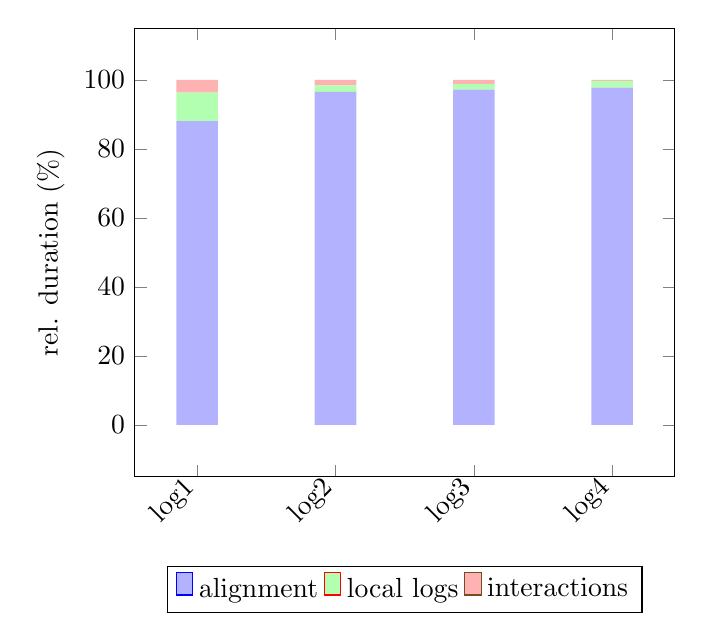
\begin{tikzpicture}
\begin{axis}[
    ybar stacked,
    ymin=0, ymax=100,
	bar width=15pt,
	%nodes near coords,
    enlargelimits=0.15,
    legend style={at={(0.5,-0.20)},
      anchor=north,legend columns=-1},
    ylabel={rel. duration (\%)},
    symbolic x coords={log1, log2, log3, log4},
    xtick=data,
    x tick label style={rotate=45,anchor=east}
    ]
    \addplot+[ybar,fill=blue!30,draw=none] plot coordinates {(log1,88.07) (log2,96.57) (log3,97.18) (log4,97.76)};
    \addplot+[ybar,fill=green!30,draw=none] plot coordinates {(log1,8.26) (log2,1.83) (log3,1.58) (log4,1.97)};
    \addplot+[ybar,fill=red!30,draw=none] plot coordinates {(log1,3.67) (log2,1.6) (log3,1.24) (log4,0.27)};
    \legend{alignment, local logs, interactions}
\end{axis}
\end{tikzpicture}
    \caption{Relative execution times}
    \label{fig:perfrel}
\end{figure}


\section{Real-life log}
Lastly, we apply the approach comparatively to a real-life event log about a loan application process from a financial institute. We show the advantages of our approach over a commercial tool and state-of-the-art ProM plugins in reasoning about conformance and performance.
The log is from the BPI Challenge 2012 \cite{bpi2012log} and contains $262,200$ events in $13,087$ cases. It is actually composed of three intertwining subprocesses. Overall, cases start with an application, then multiple offers may be sent back and forth until the application is cancelled, declined or accepted. Work events pertaining to communication between employees and applicants are interspersed in between. Since this makes the process model discovery unfeasible, we focus just on the offer subprocess by projecting the entire log onto the offer activities. Since not every case includes an offer, this leaves $5015$ cases which usually happen as follows: Offers are first selected, then created and sent. At this point, they are either sent back, and end up declined or accepted, or are cancelled and either end immediately or loop to the beginning. It is important to note here that the log was extracted from a running system and therefore contains incomplete cases.

\subsection*{Conformance}
\begin{figure}[H]
    \centering
    \includegraphics[width=0.75\textwidth]{figures/evaluation/disco_conf.png}
    \caption{Adjusted process map of the commercial tool Disco}
    \label{fig:discoconf}
\end{figure}

First, we apply the commercial tool \emph{Disco}\footnote{https://fluxicon.com/disco/}.
It uses an directly follows activity graph as a process model and cannot give direct insights into deviations because it is not executable. Due to that there is no notion of state and concurrency is not really supported.
This already limits the ability to answer conformance questions.
Disco includes a slider for filtering the directly follows relation by frequency which can be used to include rare deviations.
Figure \ref{fig:discoconf} shows this. This model incorporates the standard offer procedure but also includes new arcs which are hard to interpret.

Applying the state-of-the-art conformance checking plugin \emph{Replay a Log on Petri Net for Conformance Analysis} is shown in Figure \ref{fig:goodconf} on \autopageref{fig:goodconf}. It yields a fitness value of $0.957$ and places are sized relatively based on the number of times they are involved in non-sync moves. This means the per-place conformance has no real metric and is just comparative. The most deviations occur on the place before the split between \textsc{O\_CANCELLED} and \textsc{O\_SENT\_BACK}. The plugin tells us that there are $767$ log moves of \textsc{O\_SELECTED} and $406$ of \textsc{O\_SENT\_BACK} on that place. This alone does not allow diagnosing what exactly happened there and especially when.

We now apply our plugin to obtain more fine grained results.
\begin{figure}[H]
    \centering
    \includegraphics[width=\textwidth]{figures/evaluation/splitplace_problems.png}
    \caption{Problem view of the sink place}
    \label{fig:splitplaceproblems}
\end{figure}
The problems view in Figure \ref{fig:splitplaceproblems} of the place at the first split gives more insight into the deviations. The number of incomplete interactions increases towards the end, making the fitness drop. The regular sojourn durations also start to fade out after the 12th of February. We see that this is mainly caused by incorrectly executed event \textsc{O\_SENT}, meaning cases simply ended afterwards. This is exactly one of the variants of incomplete cases.
For the place before the \textsc{O\_SELECTED} where the loop joins in again, the swap heuristic detects that an offer is sometimes selected before the loop, specifically the silent transition after the cancellation, is executed. This happens $578$ times and is also exactly one of the common deviations from the model.

\subsection*{Performance}

\begin{figure}[H]
    \centering
    \includegraphics[width=0.75\textwidth]{figures/evaluation/disco_processmap.pdf}
    \caption{Performance view of the commercial tool Disco}
    \label{fig:discoperf}
\end{figure}

Figure \ref{fig:discoperf} shows the performance view of Disco on the standard model with average waiting times between activities. Due to not supporting concurrency, the numbers can be very misleading. There are a few different options apart from the average but a graph over time is not available.
The closest one can get is filtering the cases with the extensive filtering options to compare more specific process maps and the new averages. This is never as fine as filtering the interactions over time.

The performance view of \emph{Replay a Log on Petri Net for Performance/Conformance Analysis} in Figure \ref{fig:goodperf} on \autopageref{fig:goodperf} is somewhat equally limited. The average sojourn time of the most problematic place which is the aforementioned first split is $10.62$ days with a standard deviation of $9.61$ days. Again, we can determine that the durations must be somewhat unstable, but we have no further information.

\begin{figure}[H]
    \centering
    \includegraphics[width=\textwidth]{figures/evaluation/splitplace_perf.png}
    \caption{Sojourn duration graph over time}
    \label{fig:splitplaceperf}
\end{figure}

The performance graph for the interesting split place shown in Figure \ref{fig:splitplaceperf} clearly indicates that sojourn durations become much shorter towards the end of the observed timeframe. Together with the scatter plot in Figure \ref{fig:splitplaceproblems}, we can diagnose that there is an unnatural improvement in performance more likely caused by the falling fitness rather than actual improvements.

\begin{figure}
    \centering
    \begin{subfigure}[t]{0.475\textwidth}
    \centering
    \includegraphics[scale=0.425,angle=90]{figures/evaluation/good_model_conf.png}
    \caption{Standard conformance analysis}
    \label{fig:goodconf}
    \end{subfigure}
    ~
    \begin{subfigure}[t]{0.475\textwidth}
    \centering
    \includegraphics[scale=0.425,angle=90]{figures/evaluation/good_model_perf.png}
    \caption{Standard performance analysis}
    \label{fig:goodperf}
    \end{subfigure}
    \caption{Standard performance analysis}
\end{figure}

This evaluation showed the advantages of the most prominent features which are the timeseries of metrics. Especially the importance of localizing over time is apparent. An analysis of the exportable dataset is out of the scope of this evaluation but may lead to even more promising results.